\chapter{PHƯƠNG PHÁP THỰC HIỆN VÀ KIẾN TRÚC HỆ THỐNG}
\label{chapter:phuong_phap_thuc_hien}

Chương này trình bày chi tiết về kiến trúc tổng thể, quy trình công nghệ và các giải pháp kỹ thuật được nghiên cứu, triển khai nhằm xây dựng hệ thống trợ lý ảo thông minh hỗ trợ dạy và học môn Khoa học tự nhiên cấp Trung học cơ sở. Nội dung trọng tâm bao gồm kiến trúc hệ thống Client--Server, quy trình trích xuất và tiền xử lý dữ liệu đa phương thức (ETL Pipeline), giải pháp xử lý chuyên biệt cho công thức khoa học, luồng xử lý truy vấn tăng cường truy xuất (RAG Pipeline) kết hợp truy xuất lai và tái xếp hạng, cùng thiết kế giao diện tương tác người dùng hiện đại.

\section{Kiến trúc tổng thể hệ thống}
Hệ thống trợ lý ảo được xây dựng dựa trên mô hình phân tầng Client--Server hiện đại, đảm bảo tính tách biệt giữa logic xử lý nghiệp vụ và giao diện tương tác, bao gồm hai phân hệ chính: Phân hệ máy chủ xử lý (Backend) và Phân hệ giao diện người dùng (Frontend).

\begin{figure}[htbp]
    \centering
    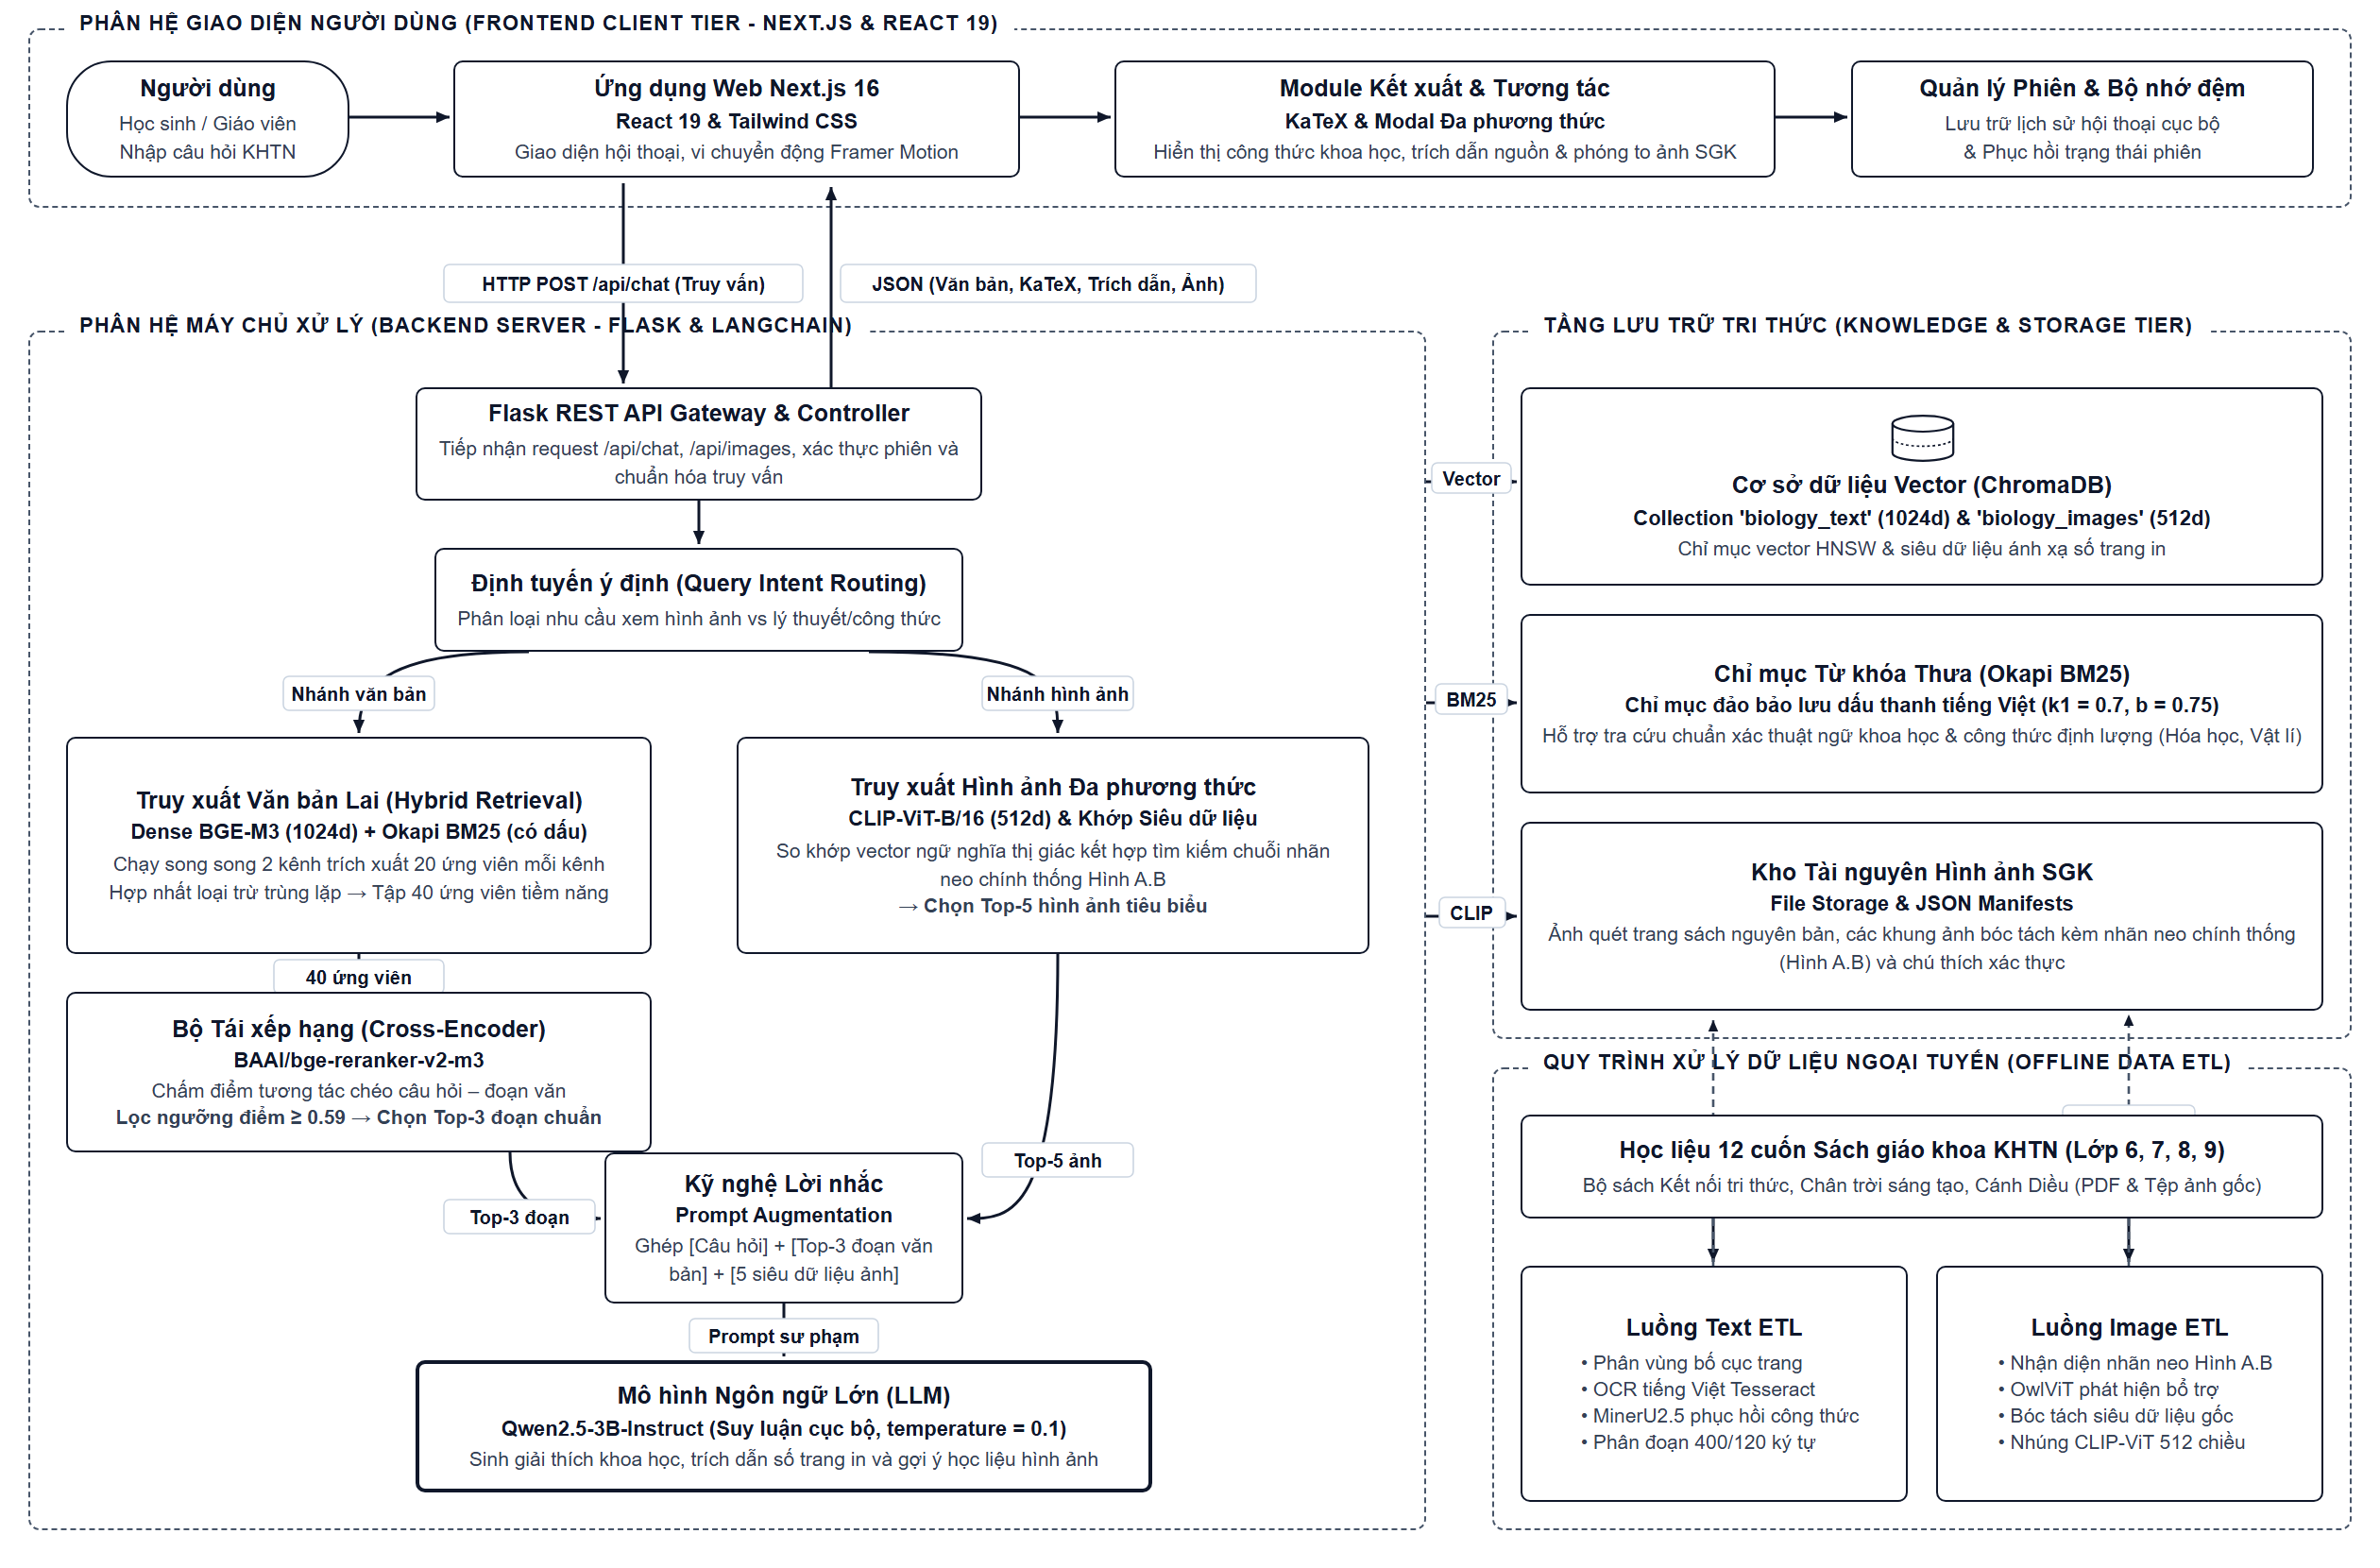
\includegraphics[width=0.9\textwidth]{src/images/chapter3/architecture.png}
    \caption{Sơ đồ kiến trúc tổng thể của hệ thống Trợ lý ảo RAG đa phương thức}
    \label{fig:system_architecture}
\end{figure}

Phân hệ Backend được hiện thực hoá bằng ngôn ngữ Python, sử dụng Flask làm nền tảng cung cấp dịch vụ giao diện lập trình ứng dụng (API Server), kết hợp cùng framework LangChain~\cite{langchain2022} đóng vai trò điều phối (orchestration) toàn diện các tác vụ xử lý ngữ cảnh, truy vấn cơ sở dữ liệu vector và triệu gọi mô hình ngôn ngữ lớn. Phân hệ Frontend được xây dựng trên nền tảng Next.js, mang lại giao diện ứng dụng một trang (Single Page Application --- SPA) mượt mà, phản hồi tức thời và tối ưu trải nghiệm người dùng.

\section{Quy trình thu thập và xử lý dữ liệu (ETL Pipeline)}
Quy trình Trích xuất, Biến đổi và Nạp dữ liệu (Extract, Transform, Load --- ETL) đóng vai trò nền tảng trong việc thiết lập Cơ sở tri thức (Knowledge Base) chuẩn mực cho hệ thống trợ lý ảo. Khác với các kho học liệu thuần văn bản, sách giáo khoa môn Khoa học tự nhiên sở hữu cấu trúc thông tin đa dạng và phức tạp: các đoạn văn lý thuyết đan xen với hệ thống \textbf{công thức định lượng} (Vật lí, Hoá học) và tài nguyên trực quan đa dạng (sơ đồ tế bào, sơ đồ giải phẫu, mạch điện, đồ thị động học, bảng biểu số liệu...). Nhằm bảo toàn trọn vẹn đặc trưng tri thức từ 12 cuốn sách giáo khoa thuộc ba bộ sách chuẩn mực hiện hành~\cite{sgk_kntt6, sgk_kntt7, sgk_kntt8, sgk_kntt9, sgk_ctst6, sgk_ctst7, sgk_ctst8, sgk_ctst9, sgk_cd6, sgk_cd7, sgk_cd8, sgk_cd9}, quy trình ETL được tổ chức thành hai luồng xử lý độc lập nhưng đồng bộ về mặt siêu dữ liệu.

\begin{table}[H]
\centering
\caption{Đặc trưng xuất bản và cấu trúc dữ liệu của ba bộ sách giáo khoa}
\label{tab:sgk_features}
\small
\begin{tabular}{lp{3.5cm}p{3.2cm}p{4cm}}
\toprule
\textbf{Bộ sách giáo khoa} & \textbf{Nhà xuất bản} & \textbf{Độ phân giải chuẩn} & \textbf{Đặc trưng bố cục \& Nhãn hình} \\
\midrule
\textbf{Kết nối tri thức} & NXB Giáo dục Việt Nam & $1094 \times 1536$ điểm ảnh & Nhãn hình chữ trắng trên nền khối màu bo góc; bố cục 1 cột kết hợp khối hoạt động khám phá \\
\textbf{Chân trời sáng tạo} & NXB Giáo dục Việt Nam & $2280 \times 3201$ điểm ảnh & Nhãn hình chữ đen in thường; mật độ sơ đồ thí nghiệm và chu trình hóa sinh cao \\
\textbf{Cánh Diều} & NXB Đại học Sư phạm & $2280 \times 3201$ điểm ảnh & Nhãn hình chữ đen in nghiêng; trình bày đa cột linh hoạt, mật độ đồ thị vật lý dày \\
\bottomrule
\end{tabular}
\end{table}

\subsection{Quy trình tiền xử lý dữ liệu văn bản (Text ETL)}
Luồng Text ETL chịu trách nhiệm nhận diện cấu trúc, trích xuất nội dung ký tự từ các trang sách giáo khoa và nạp vào cơ sở dữ liệu vector ChromaDB.

\textbf{Chuẩn hoá dữ liệu nguồn dạng tệp ảnh độ phân giải gốc:} Toàn bộ 12 cuốn sách giáo khoa được tổ chức và lưu trữ dưới dạng ảnh quét định dạng PNG (mỗi trang là một tệp ảnh độc lập) với độ phân giải nguyên bản từ nhà xuất bản (Bảng~\ref{tab:sgk_features}). Phương pháp này triệt tiêu hoàn toàn sự phụ thuộc vào các tham số ẩn khi kết xuất trung gian từ tệp PDF (như thư viện poppler), qua đó ngăn ngừa nguy cơ phải tái hiệu chuẩn các ngưỡng phân ngưỡng hình học của thuật toán phân tích bố cục mỗi khi thay đổi tham số DPI. Do ba bộ sách có sự khác biệt rõ rệt về độ phân giải chuẩn --- bộ Kết nối tri thức đạt $1094 \times 1536$ điểm ảnh, trong khi Chân trời sáng tạo và Cánh Diều đạt $2280 \times 3201$ điểm ảnh (riêng bộ Cánh Diều lớp 6 là $2480 \times 3480$ điểm ảnh) --- nên mọi ngưỡng tính toán kích thước hộp bao hình học đều được chuẩn hóa theo tỷ lệ tương đối so với chiều rộng trang thay vì sử dụng các giá trị điểm ảnh cố định.

\textbf{Xác thực số trang in chính xác thông qua tệp kê khai (Manifest):} Nhằm đảm bảo mọi trích dẫn đều có thể truy nguyên chính xác về trang sách vật lý mà học sinh đang sử dụng, mỗi cuốn sách được thiết lập một tệp kê khai ánh xạ tường minh giữa chỉ số tệp ảnh và \textit{số trang in thực tế}. Tệp manifest này được xây dựng dựa trên việc nhận dạng số trang in tại các góc trang kết hợp điều kiện ràng buộc tính đơn điệu tăng dần; các trang bìa được định danh riêng biệt và loại bỏ khỏi chỉ mục tri thức. Hệ thống chủ động dừng quy trình và đưa ra cảnh báo nếu phát hiện thiếu hụt tệp manifest, kiên quyết loại bỏ cơ chế gán nhãn suy đoán dựa trên chỉ số tệp vật lý nhằm tránh dẫn nguồn sai lệch cho người học.

Quy trình xử lý văn bản chi tiết gồm 4 bước chính:
\begin{enumerate}
    \item \textbf{Phân vùng bố cục và Nhận dạng ký tự quang học (OCR):} Thay vì áp dụng nhận dạng ký tự trên toàn bộ trang tài liệu một cách thô sơ (dễ gây xáo trộn thứ tự đọc giữa các cột văn bản, hộp thông tin phụ và hình ảnh), hệ thống tích hợp các kỹ thuật thị giác máy tính cổ điển để \textbf{phân vùng bố cục trang} (layout segmentation) thành các khối nội dung độc lập (hộp nội dung chính, khung hoạt động khám phá, thanh thông tin bên lề). Tiếp đó, thư viện Tesseract OCR~\cite{smith2007tesseract} với gói ngôn ngữ tiếng Việt (\texttt{tesseract-ocr-vie}) được áp dụng riêng trên từng vùng với chế độ phân đoạn trang (Page Segmentation Mode --- PSM) tương thích. Kết quả thực nghiệm kiểm chứng cho thấy phương pháp phân vùng trước khi OCR giúp giảm $3{,}8\%$ tỷ lệ mất mát từ ngữ so với phương pháp nhận dạng thô toàn trang.
    \item \textbf{Phân mảnh văn bản (Text Chunking):} Do giới hạn cửa sổ ngữ cảnh của các mô hình ngôn ngữ và nhằm tối ưu hoá độ chính xác của bước truy xuất, văn bản sau OCR được phân đoạn bằng công cụ \texttt{RecursiveCharacterTextSplitter} của LangChain với kích thước đoạn \texttt{chunk\_size = 400} ký tự và độ chồng lấn \texttt{chunk\_overlap = 120} ký tự. Kích thước 400 ký tự được xác định nhằm bao hàm trọn vẹn một luận điểm hoặc định nghĩa khoa học hoàn chỉnh, trong khi khoảng chồng lấn 120 ký tự đảm bảo tính liên kết ngữ nghĩa liền mạch giữa các đoạn tiếp giáp. Đặc biệt, bộ phân đoạn tuân thủ nguyên tắc giới hạn phân chia \textit{bên trong từng trang tài liệu}, do đó \textbf{tuyệt đối không có phân đoạn nào vắt ngang qua hai trang sách khác nhau}.
    \item \textbf{Nhúng ngữ nghĩa và Lập chỉ mục Vector:} Toàn bộ các đoạn văn bản được chuyển đổi thành các vector đặc trưng $1024$ chiều thông qua mô hình \texttt{BAAI/bge-m3}~\cite{chen2024bgem3} và lưu trữ trong collection \texttt{biology\_text} của ChromaDB. Mô hình này sở hữu khả năng nắm bắt ngữ cảnh dài và thấu hiểu đa ngữ vượt trội so với các kiến trúc nhúng nông ($384$ chiều) trên thang đo MTEB~\cite{muennighoff2022mteb}. Toàn bộ không gian vector được chuẩn hóa đồng nhất ở kích thước $1024$ chiều nhằm đảm bảo tính chuẩn xác cho các phép toán khoảng cách cosine trong cơ sở dữ liệu vector.
    \item \textbf{Khởi tạo chỉ mục thưa BM25 đồng bộ:} Song song với chỉ mục ngữ nghĩa theo vector đặc (Dense Index), hệ thống xây dựng một chỉ mục thưa Okapi BM25~\cite{robertson2009bm25} trên chính tập hợp các đoạn văn bản đó và chia sẻ chung định danh phân đoạn (chunk ID), sẵn sàng phục vụ kiến trúc truy xuất lai trình bày tại Mục~\ref{sec:relevance_gate}.
\end{enumerate}

\subsection{Giải pháp xử lý chuyên biệt cho công thức Hoá học và Vật lí}
\label{sec:formula_hybrid}
Một thách thức kỹ thuật đặc thù trong số hoá học liệu Khoa học tự nhiên là sự suy thoái nghiêm trọng của các công thức định lượng qua các công cụ OCR thông thường. Thực nghiệm khảo sát cho thấy mặc dù Tesseract nhận dạng tốt văn xuôi tiếng Việt, công cụ này \textbf{hầu như phá vỡ hoàn toàn các chỉ số dưới trong công thức hoá học và vật lí}: ví dụ phân tử \ce{O2} thường bị nhận dạng nhầm thành chuỗi \texttt{0,}, và \ce{CO2} biến dạng thành \texttt{CO,} hoặc \texttt{(0,}. Thống kê định lượng trên đường cơ sở nhận dạng ký tự truyền thống (baseline Tesseract OCR đơn thuần) ghi nhận tỷ lệ biến dạng so với nhận dạng đúng lên tới \textbf{256:3} ở bộ Cánh Diều, \textbf{377:3} ở Chân trời sáng tạo và \textbf{408:4} ở Kết nối tri thức; đồng thời không có bất kỳ ký tự chỉ số dưới dạng Unicode chuẩn nào tồn tại sau quá trình nhận dạng. Phân tích thực nghiệm cũng bác bỏ giả thuyết cho rằng sai số này do độ phân giải thấp của ảnh nguồn, bởi ngay cả các bộ sách có độ phân giải cao gấp đôi vẫn chịu sự suy giảm tương đương về tỷ lệ công thức lỗi.

\textbf{Lựa chọn công cụ thông qua thực nghiệm đối sánh độc lập (Bake-off):} Nhằm tìm kiếm giải pháp thay thế hiệu quả, đề tài thiết lập một tập kiểm thử chuẩn (gold set) gồm $97$ ô văn bản phân bố trên $15$ trang sách (cân đối $5$ trang cho mỗi bộ sách) được các chuyên gia đối chiếu và nhập liệu thủ công. Kết quả thử nghiệm mô hình thị giác--ngôn ngữ tiên tiến MinerU2.5 cho thấy mô hình này cải thiện vượt bậc khả năng đọc chỉ số dưới với tỷ lệ chính xác đạt $\mathbf{0{,}441}$ (cao gấp $9{,}2$ lần so với mức $0{,}048$ của Tesseract). Tuy nhiên, MinerU2.5 lại bộc lộ nhược điểm lớn ở văn xuôi tiếng Việt khi làm tăng tỷ lệ lỗi dấu thanh lên mức $\mathbf{0{,}037}$, cao hơn đáng kể so với mức $0{,}016$ của Tesseract. Do nội dung văn xuôi chiếm hơn $93\%$ dung lượng sách giáo khoa, việc thay thế hoàn toàn Tesseract bằng MinerU2.5 sẽ dẫn tới sự suy giảm nghiêm trọng về chất lượng ngữ nghĩa tiếng Việt của toàn bộ tài liệu.

\textbf{Kiến trúc xử lý lai phân cấp theo dòng (Line-level Hybrid Architecture):} Từ phát hiện trên, đề tài đề xuất giải pháp kiến trúc lai: duy trì Tesseract làm công cụ chủ đạo cho toàn bộ văn bản thông thường, đồng thời phát triển một cổng phân loại nhanh (\texttt{is\_formula\_suspect}) để quét từng dòng văn bản và phát hiện các mẫu nghi ngờ chứa công thức bị phân rã. Bộ lọc này đạt độ chính xác (Precision) $\mathbf{0{,}8654}$ và độ phủ (Recall) $\mathbf{1{,}0000}$ trên tập kiểm định gồm $89$ ô văn bản. Chỉ những dòng bị nghi ngờ lỗi mới được trích xuất ảnh tương ứng để gửi tới mô hình MinerU2.5 xử lý lại. 

Nhằm đảm bảo tính nguyên vẹn và tránh việc hệ thống tự ý chắp vá thông tin sai lệch, cơ chế ghép ngược (merging) tuân thủ nguyên tắc ràng buộc chặt chẽ: phép thay thế chỉ được kích hoạt khi số lượng thực thể khoa học do MinerU2.5 phát hiện trùng khớp hoàn toàn với số lượng vị trí suy biến do Tesseract để lại. Trường hợp không thỏa mãn điều kiện khớp số lượng, dòng văn bản sẽ được bảo lưu nguyên trạng kết quả của Tesseract. Quy trình này đã được triển khai xử lý hoàn tất trên toàn bộ $16.515$ phân đoạn của kho tri thức thực tế (ghi nhận $4\,293$ lượt ghép dòng thành công, $0$ lỗi ngoại lệ).

\subsection{Quy trình tiền xử lý dữ liệu hình ảnh (Image ETL)}
Nhằm hỗ trợ học sinh tiếp cận kiến thức thông qua các tài nguyên trực quan, luồng Image ETL được tổ chức tuần tự theo 4 giai đoạn:
\begin{enumerate}
    \item \textbf{Phát hiện khung ảnh dựa trên neo chú thích (Anchor-first Detection):} Thay vì phụ thuộc hoàn toàn vào các mô hình học sâu phát hiện vật thể (vốn dễ chịu ảnh hưởng bởi nhiễu nền của trang sách phức tạp), hệ thống ưu tiên định vị các chuỗi ký tự định danh chính thức có cấu trúc \texttt{Hình A.B} xuất hiện trên trang. Dựa trên quy ước bố cục in ấn của từng bộ sách, toạ độ của hình ảnh minh hoạ phía trên hoặc phía dưới dòng chú thích sẽ được trích xuất chính xác. Mô hình thị giác \texttt{google/owlvit-base-patch32}~\cite{minderer2022owlvit} chỉ đóng vai trò hỗ trợ phụ trợ đối với các khung ảnh đặc thù không đi kèm nhãn chú thích tiêu chuẩn. Ưu thế then chốt của giải pháp này là tính minh bạch và khả năng giải trình: mỗi khung ảnh được cắt ra đều gắn liền với một nhãn định danh chính thống trên trang sách.
    \item \textbf{Cấu hình trích xuất thích ứng theo định dạng xuất bản:} Thống kê bố cục cho thấy các bộ sách áp dụng phong cách thiết kế nhãn hình khác nhau: bộ Kết nối tri thức sử dụng nhãn \textbf{chữ trắng in trên nền khối màu bo góc} (phát hiện trung bình $23$--$28$ nhãn/30 trang qua kênh xử lý ngưỡng màu chuyên biệt); trong khi Chân trời sáng tạo và Cánh Diều sử dụng \textbf{chữ đen thông thường} ($30$--$65$ nhãn/30 trang qua kênh OCR chuẩn). Hệ thống tự động nhận diện hồ sơ bố cục (layout profile) tương ứng với từng bộ sách để áp dụng giải thuật bóc tách tối ưu, ngăn ngừa hoàn toàn hiện tượng nhầm lẫn cấu trúc.
    \item \textbf{Xây dựng siêu dữ liệu xác thực từ điểm ảnh:} Mỗi khung hình sau khi trích xuất được gắn kèm các trường siêu dữ liệu trích xuất trực tiếp từ trang sách gốc: nhãn hình (\texttt{Hình A.B}), chuỗi chú thích nội dung và các từ ngữ nhận dạng được bên trong khung ảnh. Hệ thống chủ động loại bỏ việc sử dụng các mô hình tự động sinh chú thích ảnh (Image Captioning) như Vintern-1B. Khảo nghiệm trên dữ liệu thực tế cho thấy mô hình sinh chú thích tiêu tốn tới $17{,}6$ giây/ảnh trên CPU, đồng thời bộc lộ tỷ lệ sinh ảo giác cao ($4/12$ trường hợp tự suy diễn chi tiết không có thật, và gán sai $4/4$ số hiệu hình). Việc sử dụng siêu dữ liệu xác thực từ văn bản gốc đảm bảo độ chính xác tuyệt đối và loại bỏ hoàn toàn các rủi ro sai lệch tri thức trực quan.
    \item \textbf{Lập chỉ mục đa phương thức (Multimodal Indexing):} Mỗi khung hình được mã hoá thành vector nhúng $512$ chiều thông qua mô hình liên kết ngôn ngữ -- thị giác \texttt{clip-vit-base-patch16}~\cite{radford2021clip} và lưu trữ trong collection \texttt{biology\_images} cùng siêu dữ liệu định danh, phục vụ việc tìm kiếm tương đồng đa phương thức.
\end{enumerate}

Bên cạnh quy trình tự động, hệ thống cung cấp sẵn các công cụ kết xuất dữ liệu phục vụ cơ chế chuyên gia rà soát (Human-in-the-loop), tạo điều kiện cho các chuyên gia chuyên môn hoặc người quản trị hệ thống có thể kiểm tra và hiệu chỉnh siêu dữ liệu hình ảnh khi có nhu cầu chuẩn hóa chuyên sâu.

\section{Luồng truy xuất và sinh văn bản (RAG Pipeline)}
Khi người dùng (học sinh hoặc giáo viên) nhập câu hỏi trên giao diện, hệ thống Backend tiếp nhận và điều phối luồng xử lý RAG đa phương thức theo các giai đoạn được mô tả trong Hình~\ref{fig:rag_pipeline_detail}:

\begin{figure}[htbp]
    \centering
    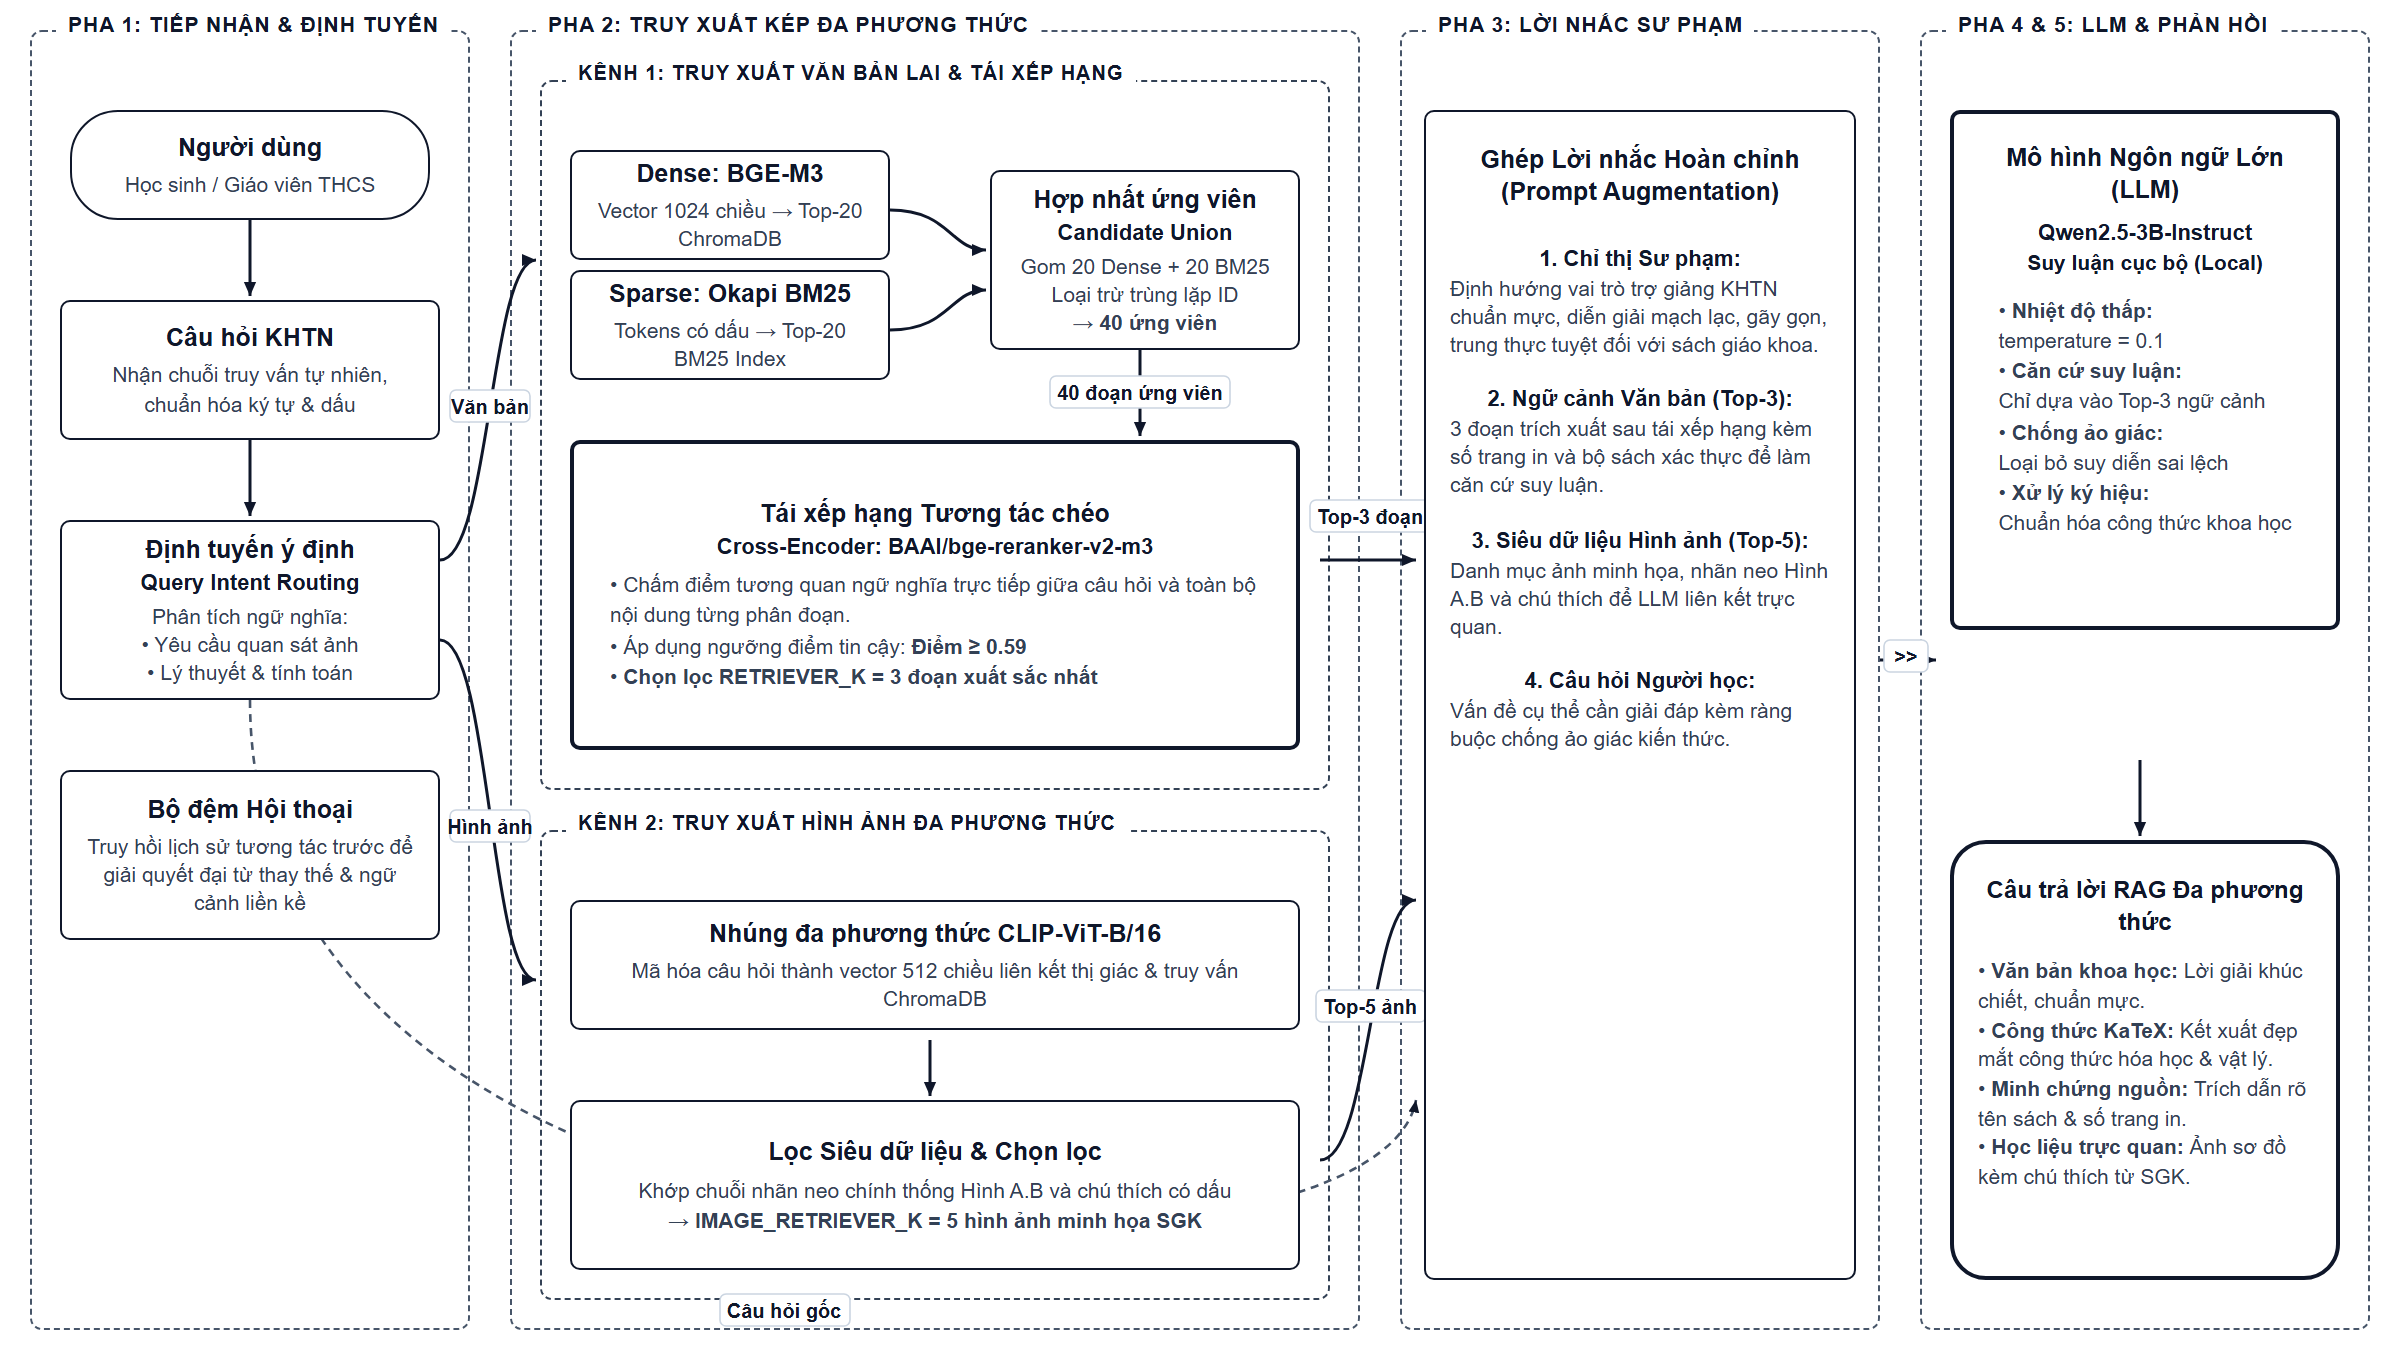
\includegraphics[width=0.65\textwidth]{src/images/chapter3/rag_pipeline.png}
    \caption{Luồng xử lý truy vấn RAG đa phương thức tại Backend}
    \label{fig:rag_pipeline_detail}
\end{figure}

\begin{enumerate}
    \item \textbf{Cơ chế truy xuất kép (Dual Retrieval):} Phía dữ liệu văn bản, câu hỏi được chuyển đồng thời qua kênh tìm kiếm ngữ nghĩa vector và kênh tìm kiếm từ khoá BM25 (mỗi kênh trích chọn $20$ ứng viên ban đầu). Tập hợp ứng viên sau đó được hợp nhất và tái xếp hạng chuyên sâu bằng mô hình cross-encoder để chọn ra $\mathtt{RETRIEVER\_K = 3}$ đoạn văn bản có độ liên quan cao nhất. Phía dữ liệu hình ảnh, hệ thống trích chọn $\mathtt{IMAGE\_RETRIEVER\_K = 5}$ hình ảnh tiêu biểu dựa trên sự kết hợp giữa độ tương đồng vector CLIP và phép so khớp chuỗi siêu dữ liệu có dấu.
    \item \textbf{Kỹ nghệ thiết kế lời nhắc (Prompt Engineering):} Ngữ cảnh văn bản được chọn lọc sẽ được liên kết đồng bộ với thông tin mô tả của các hình ảnh tìm được. Lời nhắc (Prompt) được thiết kế theo cấu trúc sư phạm chuyên biệt, định hướng mô hình ngôn ngữ lớn đóng vai trò người trợ giảng Khoa học tự nhiên chuẩn mực, trả lời gãy gọn, mạch lạc và tuyệt đối trung thành với ngữ cảnh tài liệu được cung cấp.
    \item \textbf{Sinh câu trả lời (Text Generation):} Mô hình Qwen2.5-3B-Instruct~\cite{qwen25_2024} tiếp nhận lời nhắc hoàn chỉnh để sinh ra câu trả lời cuối cùng. Siêu tham số nhiệt độ được thiết lập ở mức thấp (\texttt{temperature = 0.1}) nhằm tối đa hóa tính xác thực của câu trả lời, hạn chế tối đa tính ngẫu nhiên và ngăn ngừa hiện tượng suy diễn sai lệch kiến thức khoa học.
\end{enumerate}

\subsection{Cơ chế định tuyến theo ý định truy vấn (Query Intent Routing)}
Không phải mọi tương tác của học sinh đều đòi hỏi đồng thời cả văn bản lý thuyết lẫn tài liệu hình ảnh. Module định tuyến ý định (\texttt{query\_intent}) thực hiện phân tích cấu trúc ngữ nghĩa của câu hỏi trước khi kích hoạt quy trình truy xuất. Khi phát hiện các truy vấn thể hiện rõ ý định quan sát trực quan (chứa các cụm từ như "cho xem hình", "sơ đồ cấu tạo", "biểu đồ minh hoạ"), hệ thống sẽ ưu tiên tối đa luồng truy xuất hình ảnh. Ngược lại, đối với các câu hỏi bản chất lý thuyết trừu tượng hoặc bài tập tính toán, luồng văn bản sẽ đóng vai trò chủ đạo nhằm loại bỏ các hình ảnh gây nhiễu ngữ cảnh.

\subsection{Truy xuất lai thưa -- dày và cơ chế tái xếp hạng}
\label{sec:relevance_gate}
Truy xuất ngữ nghĩa vector (Dense Retrieval) sở hữu khả năng bao quát ý nghĩa tương đồng xuất sắc, song lại gặp bất lợi lớn trước các yêu cầu so khớp định danh chính xác vốn rất phổ biến trong môn Khoa học tự nhiên: ví dụ truy vấn về phân tử \ce{CO2} hoặc định luật Boyle--Mariotte đòi hỏi sự xuất hiện chuẩn xác của chuỗi ký hiệu thay vì xấp xỉ ngữ nghĩa. Ngược lại, truy xuất từ khóa thưa (Sparse Retrieval) lại mất khả năng liên kết khi học sinh sử dụng ngôn ngữ diễn đạt khác biệt với nguyên văn sách giáo khoa. Hệ thống giải quyết sự đánh đổi này thông qua kiến trúc \textbf{Truy xuất lai (Hybrid Retrieval)}: chạy song song kênh vector \texttt{bge-m3} và kênh Okapi BM25~\cite{robertson2009bm25} trên cùng cơ sở dữ liệu phân đoạn, sau đó tiến hành hợp nhất kết quả.

\subsubsection{Tối ưu hóa chỉ mục BM25 và chuẩn hoá công thức}
Thuật toán Okapi BM25 được tự hiện thực hoá trong hệ thống nhằm hỗ trợ việc tinh chỉnh động hai siêu tham số $k_1$ và $b$ ngay tại thời điểm xử lý truy vấn. Quá trình quét lưới thực nghiệm $5 \times 5$ đã xác định bộ tham số tối ưu đạt $k_1 = 0{,}7$ và $b = 0{,}75$.

Một phát hiện thực nghiệm có ý nghĩa khoa học quan trọng là: thuật toán tách từ \textbf{bảo lưu dấu thanh tiếng Việt} đạt hiệu năng vượt trội so với giải pháp loại bỏ dấu thanh (chỉ số MRR đạt $0{,}820$ so với $0{,}755$). Việc loại bỏ dấu thanh dẫn tới hiện tượng đồng âm sai lệch nghiêm trọng giữa các hư từ và các khái niệm khoa học then chốt (ví dụ: \textit{khí} biến thành \textit{khi}, \textit{độ} thành \textit{do}, \textit{lá} thành \textit{la}, \textit{đá} thành \textit{da}).

Đối với các công thức khoa học, hệ thống áp dụng cơ chế \textbf{chuẩn hoá ký hiệu ở phía truy vấn và phía chỉ mục thưa, tuyệt đối không chỉnh sửa nội dung văn bản lưu trữ gốc}. Thử nghiệm trên $12$ công thức hóa học tiêu biểu cho thấy số phân đoạn chính xác lọt vào top-10 tăng từ $6$ lên $97$ đoạn, và số câu truy vấn tìm được tài liệu đích tăng ngoạn mục từ $1/12$ lên $11/12$.

\subsubsection{Quy trình hợp nhất và Tái xếp hạng bằng Cross-Encoder}
Quy trình truy xuất được tổ chức tuần tự: \textbf{Truy xuất song song $\rightarrow$ Hợp nhất danh sách $\rightarrow$ Tái xếp hạng}. Bước tái xếp hạng sử dụng mô hình cross-encoder \texttt{BAAI/bge-reranker-v2-m3} cùng họ BGE, thực hiện tính toán lại điểm số liên quan trên toàn bộ tập ứng viên hợp nhất từ hai kênh.

Các phân tích thực nghiệm tại Chương~\ref{chapter:thuc_nghiem_danh_gia} đã chứng minh rằng việc áp dụng thêm cổng lọc dựa trên khoảng cách tương đối trước bước tái xếp hạng không mang lại cải thiện, thậm chí làm suy giảm độ phủ (Recall@10 giảm từ $1{,}000$ xuống $0{,}890$) do loại bỏ nhầm các đoạn tài liệu đúng ở các câu hỏi phức hợp nhiều ý. Thay vào đó, việc thiết lập \textbf{ngưỡng điểm số tuyệt đối} tại bộ tái xếp hạng mang lại hiệu quả phân loại tin cậy hơn hẳn. Do đó, cấu hình tối ưu mặc định của hệ thống được xác lập là: \textbf{Truy xuất lai, kích hoạt tái xếp hạng bằng cross-encoder và vô hiệu hoá cổng lọc khoảng cách tương đối}.

\begin{table}[H]
\centering
\caption{Tổng hợp siêu tham số vận hành của hệ thống trợ lý ảo}
\label{tab:hyperparams}
\small
\begin{tabular}{lp{6.2cm}c}
\toprule
\textbf{Thành phần} & \textbf{Ý nghĩa kỹ thuật} & \textbf{Giá trị cấu hình} \\
\midrule
\texttt{EMBEDDING\_DIM} & Số chiều không gian vector BGE-M3 & $1024$ \\
\texttt{CLIP\_DIM} & Số chiều không gian vector hình ảnh CLIP & $512$ \\
\texttt{CHUNK\_SIZE} & Kích thước phân đoạn văn bản & $400$ ký tự \\
\texttt{CHUNK\_OVERLAP} & Khoảng trượt liên kết giữa các đoạn liền kề & $120$ ký tự \\
\texttt{BM25\_K1} & Tham số bão hòa tần suất từ khóa BM25 & $0{,}7$ \\
\texttt{BM25\_B} & Tham số chuẩn hóa độ dài văn bản BM25 & $0{,}75$ \\
\texttt{TOP\_K\_CANDIDATES} & Số ứng viên sơ tuyển mỗi kênh (BM25, Dense) & $20$ \\
\texttt{RETRIEVER\_K} & Số đoạn văn bản chọn lọc sau tái xếp hạng & $3$ \\
\texttt{IMAGE\_RETRIEVER\_K} & Số khung hình trích chọn đa phương thức & $5$ \\
\texttt{RERANK\_SCORE\_MIN} & Ngưỡng điểm tối thiểu của Cross-Encoder & $0{,}59$ \\
\texttt{LLM\_TEMPERATURE} & Nhiệt độ sinh văn bản của Qwen2.5 & $0{,}1$ \\
\texttt{RANDOM\_SEED} & Hạt giống ngẫu nhiên tái lập thực nghiệm & $42$ \\
\bottomrule
\end{tabular}
\end{table}

\section{Thiết kế giao diện người dùng tương tác (Frontend)}
Giao diện ứng dụng được thiết kế tối ưu hóa cho trải nghiệm học tập của học sinh Trung học cơ sở, phát triển trên nền tảng \textbf{Next.js 16.2.6} và thư viện \textbf{React 19.2.4}.

Các công nghệ giao diện chính bao gồm:
\begin{itemize}
    \item \textbf{Tailwind CSS:} Đảm bảo thiết kế giao diện hiện đại, trực quan, thân thiện với lứa tuổi học đường và tương thích hoàn hảo trên đa dạng thiết bị (Responsive Design).
    \item \textbf{Framer Motion:} Hiện thực hoá các chuyển động vi mô (micro-animations) mượt mà khi người dùng tương tác gửi nhận câu hỏi, tạo cảm giác thân thiện như đang trao đổi trực tiếp cùng một gia sư chuyên môn.
    \item \textbf{Hiển thị công thức khoa học bằng KaTeX:} Tích hợp thư viện KaTeX kết hợp cơ chế tự động phân tích và chuyển đổi các ký tự hóa học phẳng (như \texttt{H2SO4}) sang định dạng ký hiệu chuẩn khoa học (\ce{H2SO4}). Quá trình này tra cứu bảng tuần hoàn $118$ nguyên tố hoá học để đảm bảo chỉ chuyển đổi khi chuỗi ký hiệu hợp lệ, tránh biến đổi nhầm các từ ngữ văn bản thông thường.
    \item \textbf{Minh bạch hóa học liệu qua khối trích dẫn chuyên biệt:} Hệ thống máy chủ Backend phân tách tường minh giữa nội dung văn bản câu trả lời (\texttt{answer\_text}) và trường siêu dữ liệu trích dẫn nguồn có cấu trúc (\texttt{citations} gồm tên bộ sách, số trang và mục bài học). Giao diện người dùng hiển thị riêng biệt khối trích dẫn này ngay bên dưới câu trả lời, giúp học sinh và giáo viên dễ dàng đối chiếu trực tiếp với trang sách giáo khoa tương ứng.
    \item \textbf{Cơ chế phục vụ tài nguyên hình ảnh trực tiếp từ máy chủ:} Thay vì sao chép thủ công kho dữ liệu hình ảnh sang phía máy khách, hệ thống xây dựng tuyến đường dẫn (route) phục vụ hình ảnh động từ máy chủ Backend. Giải pháp này đảm bảo tính đồng bộ dữ liệu hình ảnh và tối ưu hóa hiệu năng truyền tải trên mạng Internet.
\end{itemize}

\subsection{Một số giao diện tiêu biểu của ứng dụng}
Hình~\ref{fig:fe_overview} minh họa các màn hình chức năng chính trong luồng trải nghiệm của người dùng: từ quá trình đăng nhập hệ thống, khung đối thoại đặt câu hỏi cho tới màn hình hiển thị câu trả lời tích hợp công thức KaTeX và hình ảnh trích xuất. Hình~\ref{fig:fe_image_detail} thể hiện tính năng chi tiết của hệ thống đa phương thức: cho phép người dùng phóng to hình ảnh minh họa và kiểm tra trực tiếp trang sách giáo khoa gốc do hệ thống trích xuất.

\begin{figure}[H]
    \centering
    \begin{subfigure}[t]{0.48\textwidth}
        \centering
        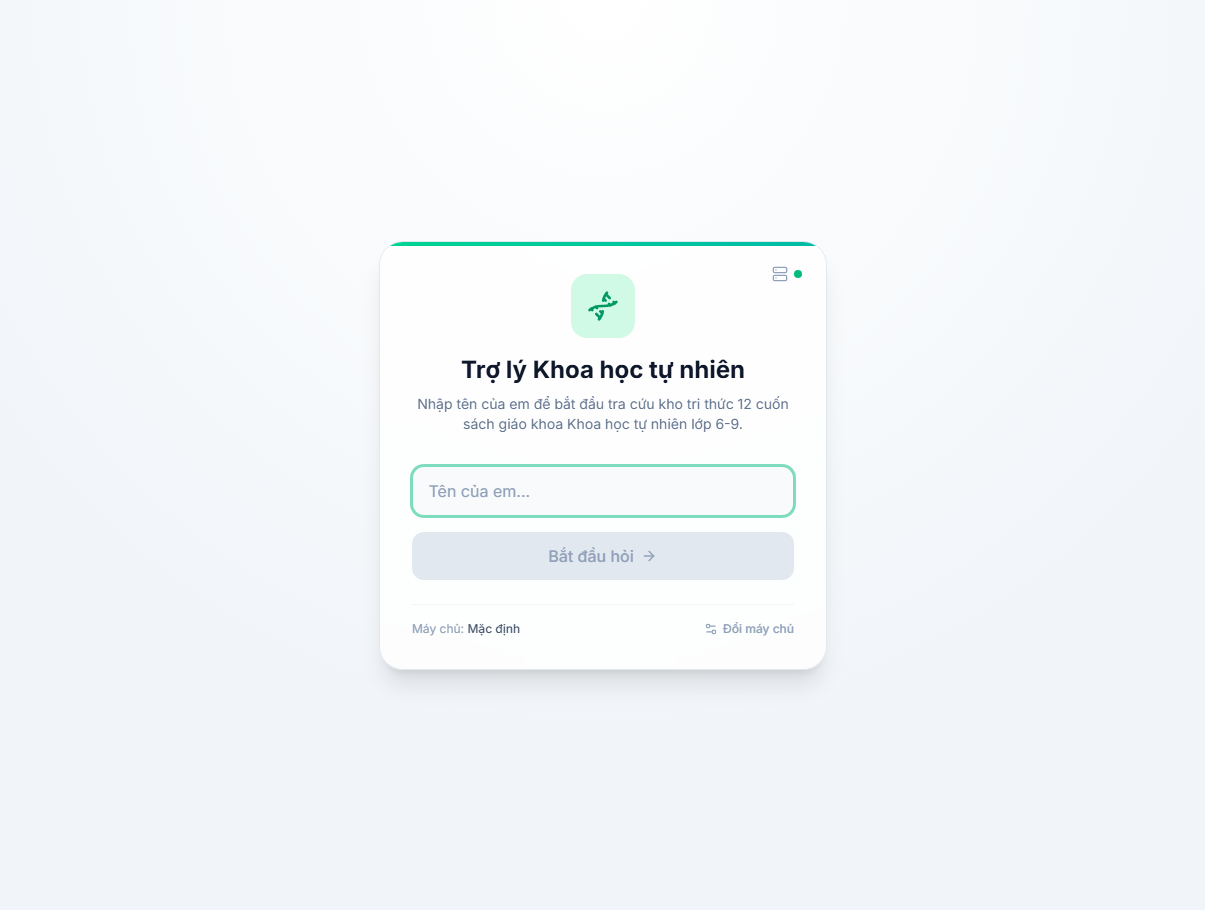
\includegraphics[width=\linewidth]{src/images/chapter3/fe-login.png}
        \caption{Màn hình đăng nhập}
        \label{fig:fe_login}
    \end{subfigure}\hfill
    \begin{subfigure}[t]{0.48\textwidth}
        \centering
        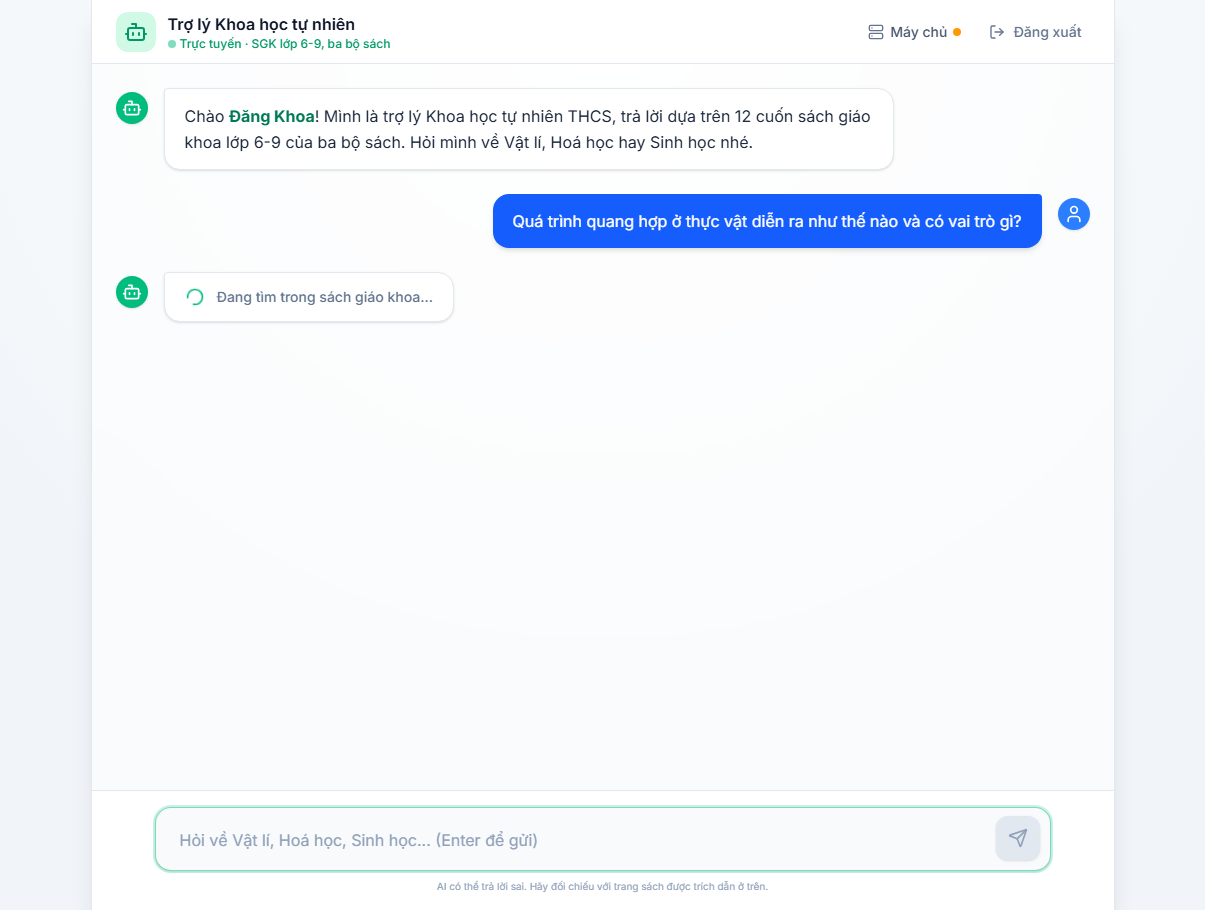
\includegraphics[width=\linewidth]{src/images/chapter3/fe-ask-question.png}
        \caption{Màn hình đặt câu hỏi}
        \label{fig:fe_ask}
    \end{subfigure}

    \vspace{1em}
    \begin{subfigure}[t]{0.48\textwidth}
        \centering
        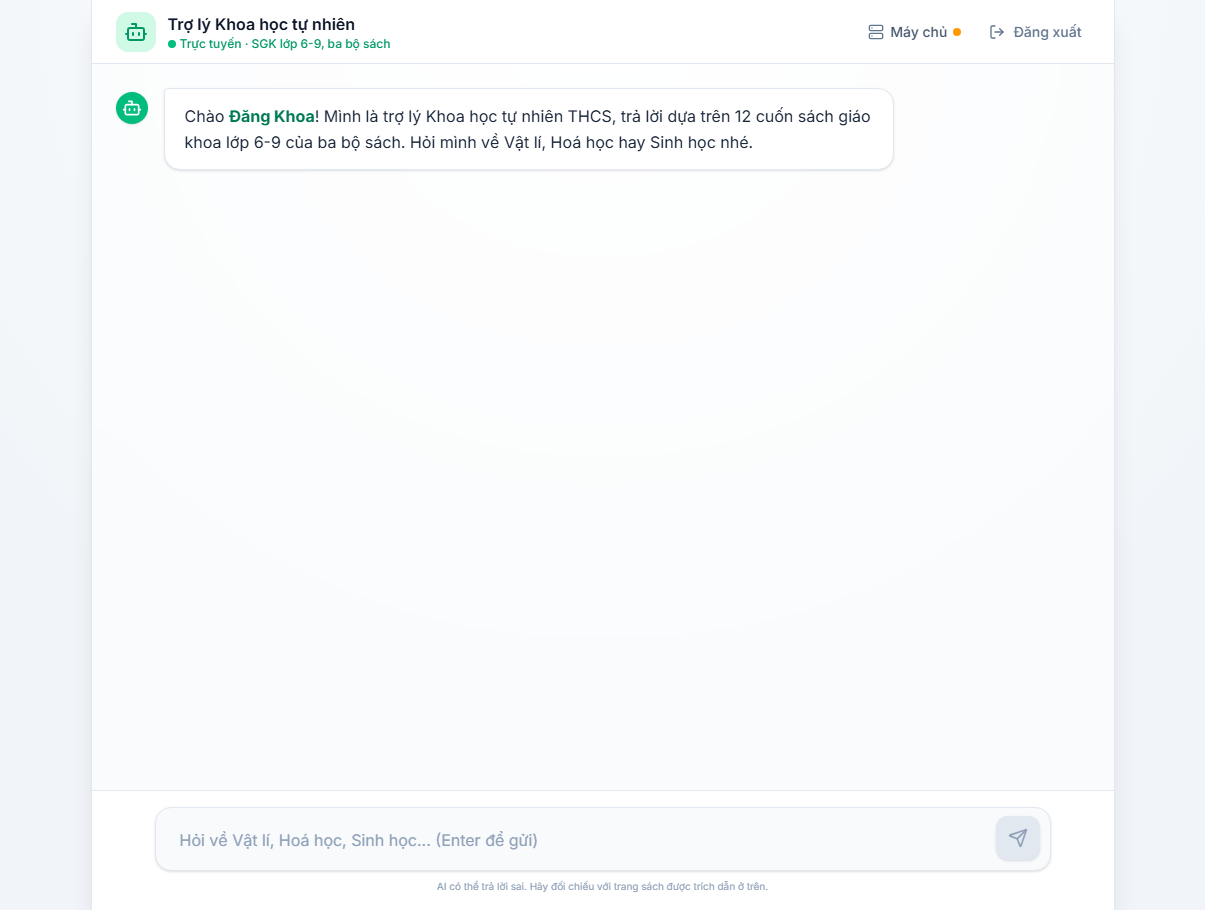
\includegraphics[width=\linewidth]{src/images/chapter3/fe-chatbox.png}
        \caption{Khung tương tác trò chuyện}
        \label{fig:fe_chatbox}
    \end{subfigure}\hfill
    \begin{subfigure}[t]{0.48\textwidth}
        \centering
        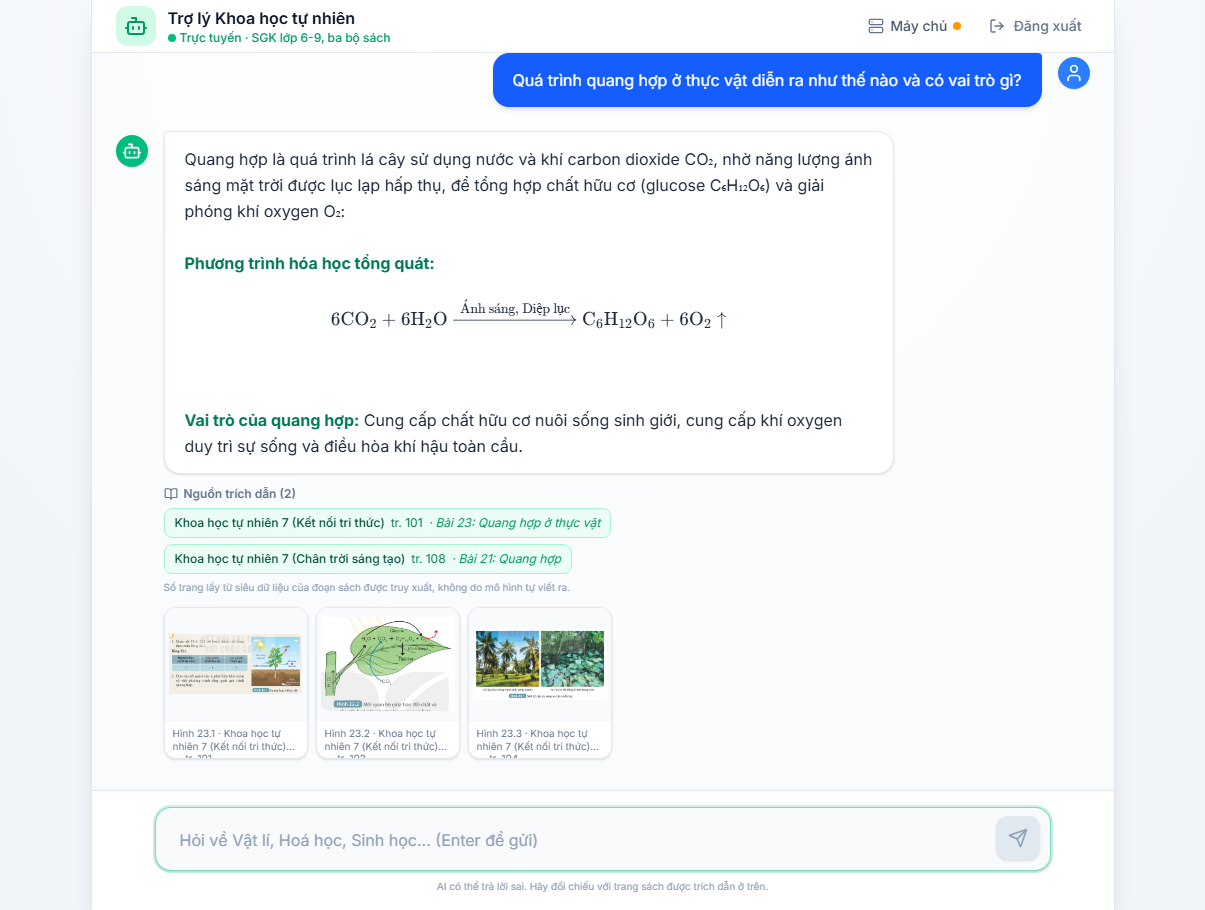
\includegraphics[width=\linewidth]{src/images/chapter3/fe-response.png}
        \caption{Hiển thị câu trả lời và trích dẫn}
        \label{fig:fe_response}
    \end{subfigure}
    \caption{Các màn hình chính của giao diện trợ lý ảo Khoa học tự nhiên.}
    \label{fig:fe_overview}
\end{figure}

\begin{figure}[H]
    \centering
    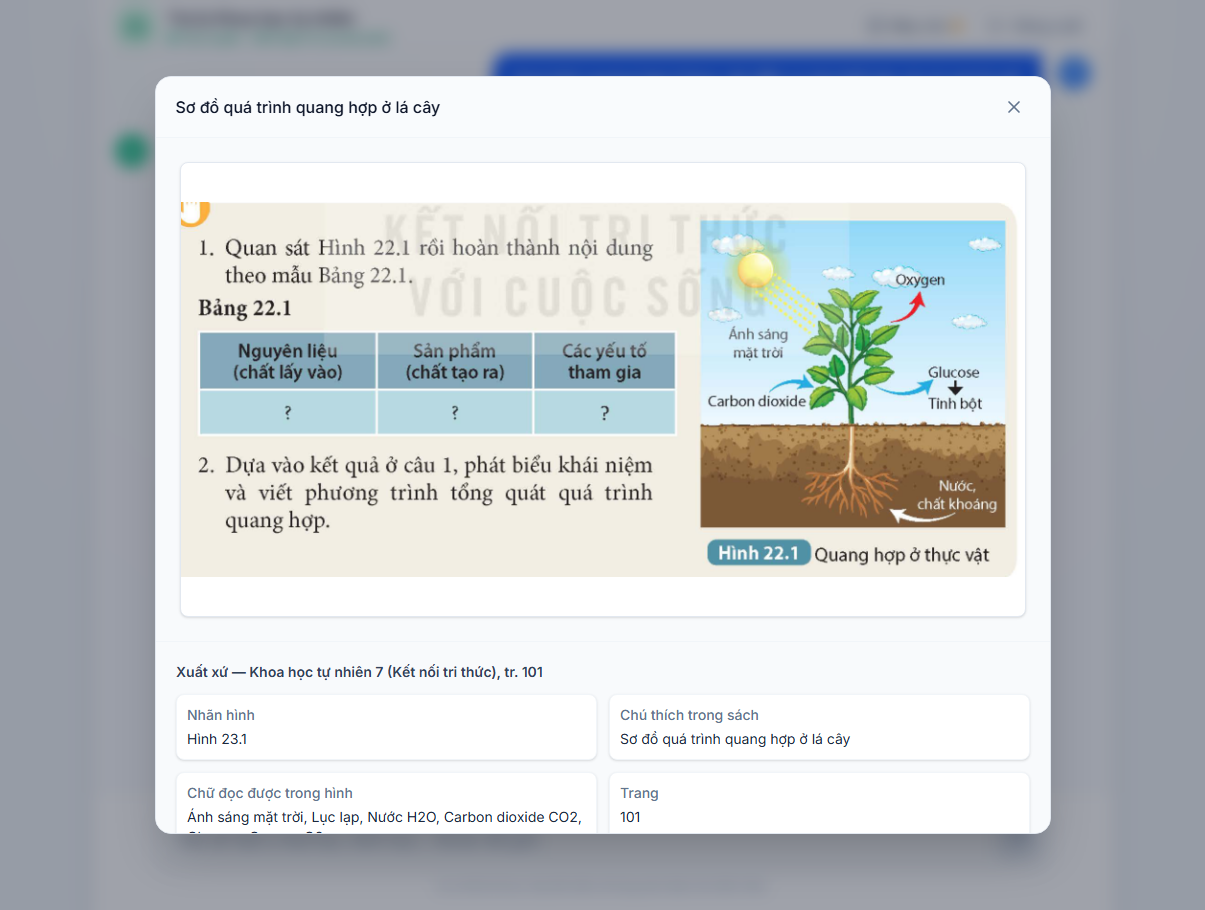
\includegraphics[width=0.75\textwidth]{src/images/chapter3/fe-image-detail.png}
    \caption{Chi tiết hình ảnh minh hoạ kèm trang sách gốc do hệ thống truy xuất.}
    \label{fig:fe_image_detail}
\end{figure}
